\chapter{Time and energy measurements} \label{ch:timing}
Substituting photomultiplier tubes or avalanche photodiodes with SiPMs in some applications could be a possible way to save space, funds, and avert the dependence on high voltage power supplies. Some of these applications, i.e. timing and energy measurements, were tested by mounting different SiPM-boards to plastics and crystals.     
\section{Signal shaping} \label{ch5:signal_shaping}
\begin{figure}[b!]
	\subfloat[Single SiPM with mask and optical grease] {\includegraphics[width=0.4\textwidth]{./pictures/plastic/SiPM_grease.jpg}}
	\hfill
	\subfloat[Mounted SiPM-boards on the plastic scintillator] {\includegraphics[width=0.4\textwidth]{./pictures/plastic/plastic_measurement.jpg}}
	\hfill
	\caption[Plastic scintillator measurement]{Mechanical setup for the efficiency and timing measurement with a plastic scintillator (wrapped, with graph paper) and \sr{} source (blue bar). A schematic can be found in figure \ref{fig:ch5:scheme_counting}.}
	\label{pic:ch5:plastic}
\end{figure}
The dark count rate measurements showed that the signal response is different for the board configurations. To obtain more information about the actual signal shape, the three configurations were mounted consecutively on opposing sides of a $\SI{25.50}{\centi\meter}\times\SI{12.25}{\centi\meter}$ plastic scintillator plate \tit{EJ-248M} from \tit{ELJEN} (see table \ref{ch2:tab:characteristics}) with cut edges and a thickness of $\SI{10}{\milli\meter}$ (a detailed schematic can be found in \ref{ap:C:plastic}). This design was chosen for measuring cosmic muons for the project \tit{Cosmic Radiation: Measuring Cosmic Muons with the Raspberry Pi} \cite{schauer_projekt}, because this shape provides a large area with a ``pseudo" light-guide to the more narrow edges where the SiPM boards will be attached.\par   
The plastic detector was wrapped with eight layers of Teflon foil and then covered with opaque black foil. For mounting, the SiPM boards were equipped with a thick rubber mask to fill the spacing between the diodes. Onto this mask a reflective foil was attached. Optical grease was carefully spread over each SiPM to grant good optical coupling with the scintillator material. The connection between board and plastic was fixed with black tape, an electrical connection was established via a pin header for the cathode and anode contacts. This setup can be see in figure \ref{pic:ch5:plastic}, a schematic is shown in figure \ref{fig:ch5:scheme_counting}, for more pictures see appendix \ref{ap:C:pictures}. A ``Bias T" was built for reading out the raw signal (see figure \ref{fig:ch5:bias_t}).  \par
\begin{figure}[t!]
	\floatbox[{\capbeside\thisfloatsetup{capbesideposition={left,center},capbesidewidth=0.65\linewidth}}]{figure}[\FBwidth]
	{\caption[``Bias T"]{``Bias T" for reading out the raw signal. The bias voltage (DC) is applied between anode (positive) and cathode (ground) for reverse biasing. A series resistor $R=\SI{10}{\kilo\ohm}$ is placed between anode and power supply, a capacitor $C=\SI{100}{\nano\farad}$ is placed between resistor and signal output and decouples the AC signal of the SiPM from the DC biasing   }    
		\label{fig:ch5:bias_t}}
	{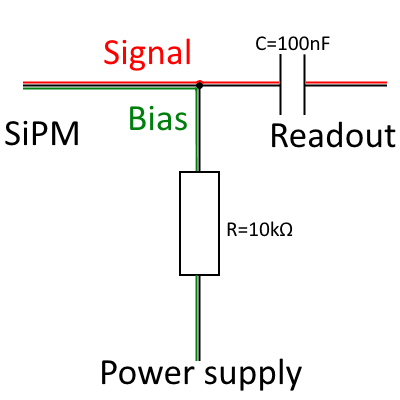
\includegraphics[width=0.3\textwidth]{./graphics/ch5/biast.png}}
\end{figure}
\begin{figure}[b!]
	\subfloat[Raw signal of the different configurations: blue (4x1 hybrid), red (4x1 parallel), green (1x1 single)] {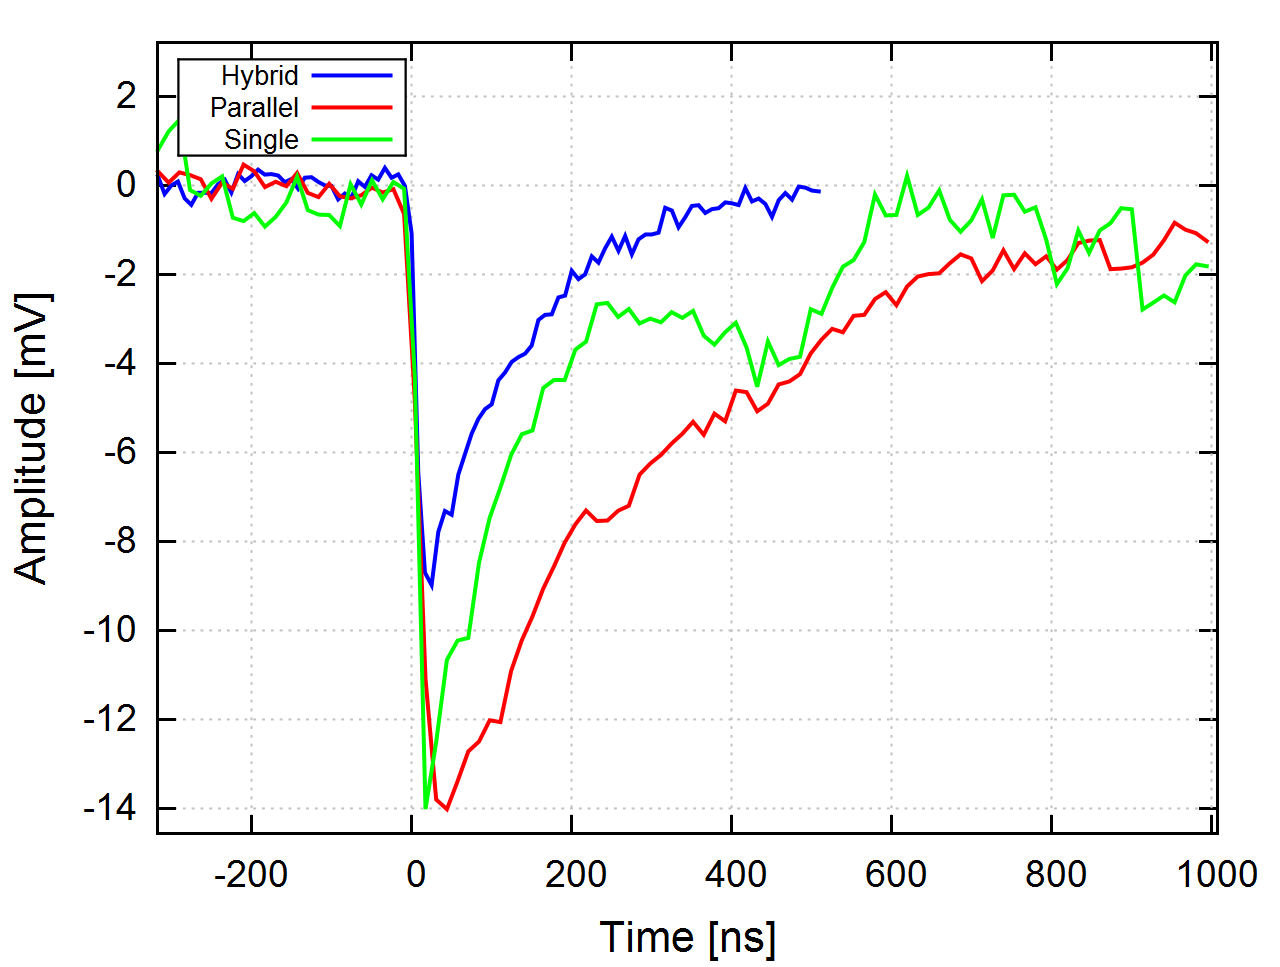
\includegraphics[width=0.49\textwidth]{./plots/signal/raw.png}}
	\hfill
	\subfloat[Amplified signal of blue (4x1 hybrid), red (4x1 parallel), green (1x1 single) with utilized photonique preamplifier] {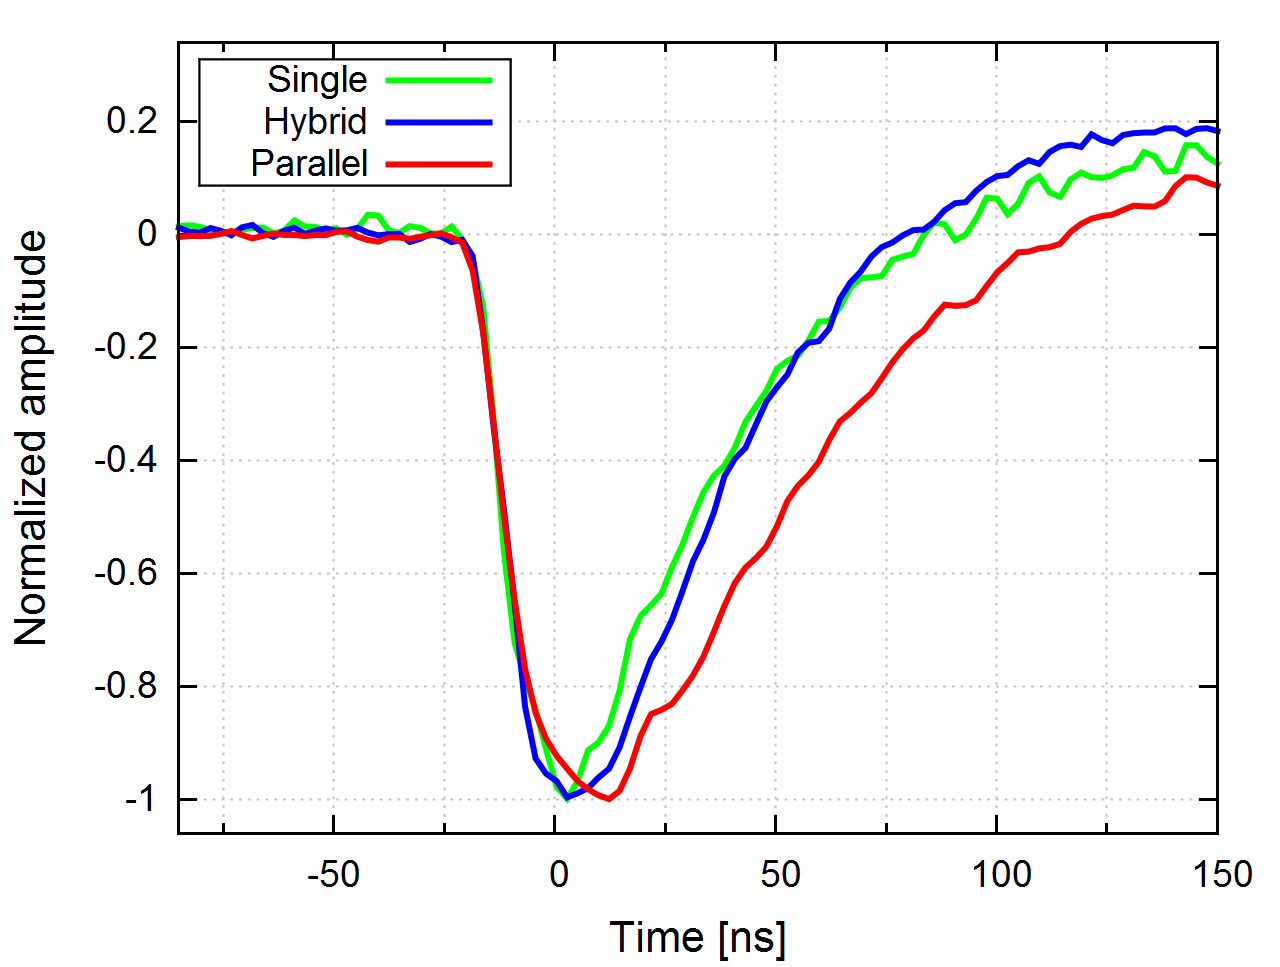
\includegraphics[width=0.49\textwidth]{./plots/signal/amp.png}}
	\hfill
	\caption[Signal shaping]{Raw and amplified signals of different SiPM configurations.}
	\label{fig:ch5:signals}
\end{figure}
With the oscilloscope used before (\tit{LeCroy Waverunner}), waveforms of the raw signals of the different SiPM configurations were acquired. For this, the SiPMs were powered with a four-channel bias source from \tit{Hameg} via the ``Bias T", the signals were fed directly to the oscilloscope. For measuring the amplified signals, the Bias T's were substituted with the \tit{photonique} preamplifiers. It was observed, that the connection between SiPM-board and preamplifier had to be as short as possible to avoid ringing and an increased noise. This was solved by directly connecting the preamp via a pin header. The bias voltage was set to $U_B=\SI{30}{\volt}$ and the power supply for the preamps was set to $U_P=\SI{5}{\volt}$. The pictures can be seen in figure \ref{fig:ch5:signals}. 
It appears that the signal amplitude of the single and parallel configurations are nearly equal, whereas the amplitude of the hybrid board is roughly half in size. Also, the baseline noise for the hybrid and parallel configurations seem to be less fluctuating. The signal rise time, which is in order of some nanoseconds, can be compared by normalizing the pulse height: the parallel configuration shows the longest rise time, the hybrid configuration the fastest. The single SiPM lies right in between. For timing, the hybrid configuration might be the most valid candidate. Even better timing can be achieved by driving the SiPMs in series, done by the PANDA Barrel-TOF detector \cite{SciTil}, but this necessitates $N$ times the bias voltage of a single SiPM, where $N$ is the number of SiPMs in series. This configuration is not considered in this thesis because of its necessity of using high voltage.   


\section{Efficiency measurements}
As a preparation for the upcoming timing measurement, the efficiency of the setup with the thin plastic scintillator plate was measured. The investigations undertaken in the last section confirmed that the hybrid configuration has the fastest rise time, so two hybrid boards were mounted to the scintillator plate used before.
\begin{figure}[b]
	\centering
	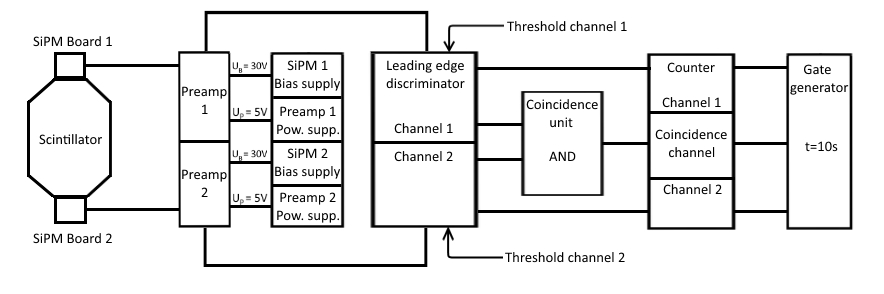
\includegraphics[width=1\linewidth]{./graphics/ch5/scheme_spatial.png}
	\caption[Schematic of the efficiency measurement]{Setup of the efficiency measurement.}
	\label{fig:ch5:scheme_counting}
\end{figure}
The experimental setup can be seen in figure \ref{fig:ch5:scheme_counting}: a four-channel power supply (Hameg HMP4040) biases the two hybrid boards with $U_{B}=\SI{30}{\volt}$ and the photonique preamplifiers with $U_{P}=\SI{5}{\volt}$. The amplified signals of the channels one and two were then discriminated by a leading edge discriminator (Lecroy 623B, TH$_1=\SI{-450}{\milli\volt}$, TH$_2=\SI{-477}{\milli\volt}$), the threshold levels TH were set to satisfy the expected count rate of cosmic muons (approximately $\SI{200}{\per\second\per\meter\squared}$ \cite{PDG}). The output of the discriminator was tracked by a counter (Uni Bonn) which was gated by a gate generator (Lecroy 222) to count the signals for $\SI{10}{\second}$. A coincidence unit (Caen N455) provided the signal to count coincident signals. \par 
A \sr{} source ($\beta^{-}$-emitter) was used to produce scintillation light. An aluminum block with a small bore was used as a collimator to guide and center the emitted electrons. For positioning, graph paper was attached to the scintillator (again, see \ref{pic:ch5:plastic}). \par
The measurement positions are show in figure \ref{fig:ch5:efficiency}. The heat map plots for the count rate show two maxima: one right in front of the SiPMs, the other on the y-axis some centimeters in front of the detectors, beginning half the way down from the center of the scintillator to the mounted boards. This region of high count rate is limited to some square centimeters and is oval shaped. The count rate in the other regions of the plastic is nearly constant, except from the very edges and corners, and right in front of the respective opposite detector, where the rate drops. The results for detector one and two are similar but not identical: detector one seems to be less effective in counting compared to detector two, which shows a more symmetric shape. The second maximum might be explained by the special shape of the cut corners, so the photons generated at this position might get reflected to the detectors. \par 
In discussing the coincident count rate, the asymmetry can be found again: the rate right in front of detector two is nearly twice as high as in front of detector one. The maxima appear again at the same positions, the rate is highest on the y-axis and decreases for positions moving along the x-axis. For events right in front of one board, the coincident count rate is apparently given by the count rate of the opposite board. \par 
Although one of the two detectors seems to have some performance issues, the coincident count rate for most of the positions, a square from -5$\si{\centi\meter}$ to +5$\si{\centi\meter}$ on the x-axis and -9$\si{\centi\meter}$ to +9$\si{\centi\meter}$ on the y-axis, is valid for using this setup for measuring cosmic muons (two detectors are used to avert detecting fake events). The time resolution will be discussed in the section following.

\section{Time resolution measurements}

For certain applications like propagation time measurements or positioning, timing properties are important. As section \ref{ch5:signal_shaping} has shown, the hybrid configuration is a valid candidate for timing applications. The time resolution and propagation time was measured for the setup used in last section. \par 
\begin{figure}[h!]
	\subfloat[Measurement positions] {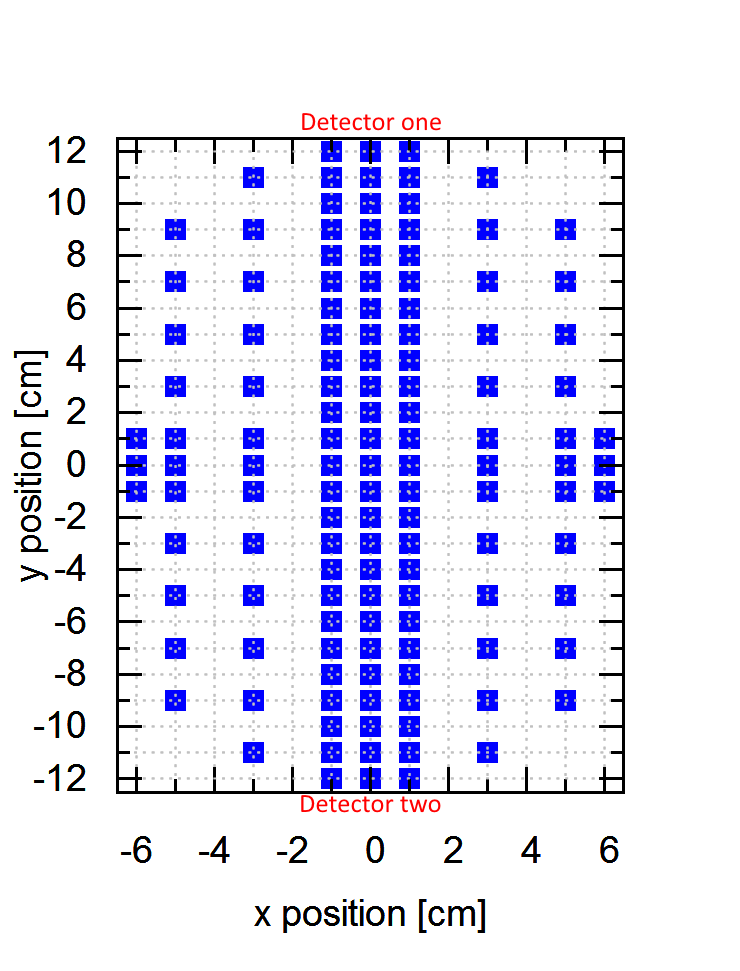
\includegraphics[width=0.4\textwidth]{./plots/spatial/aufnahme_punkte.png}}
	\hfill
	\subfloat[Detector one] {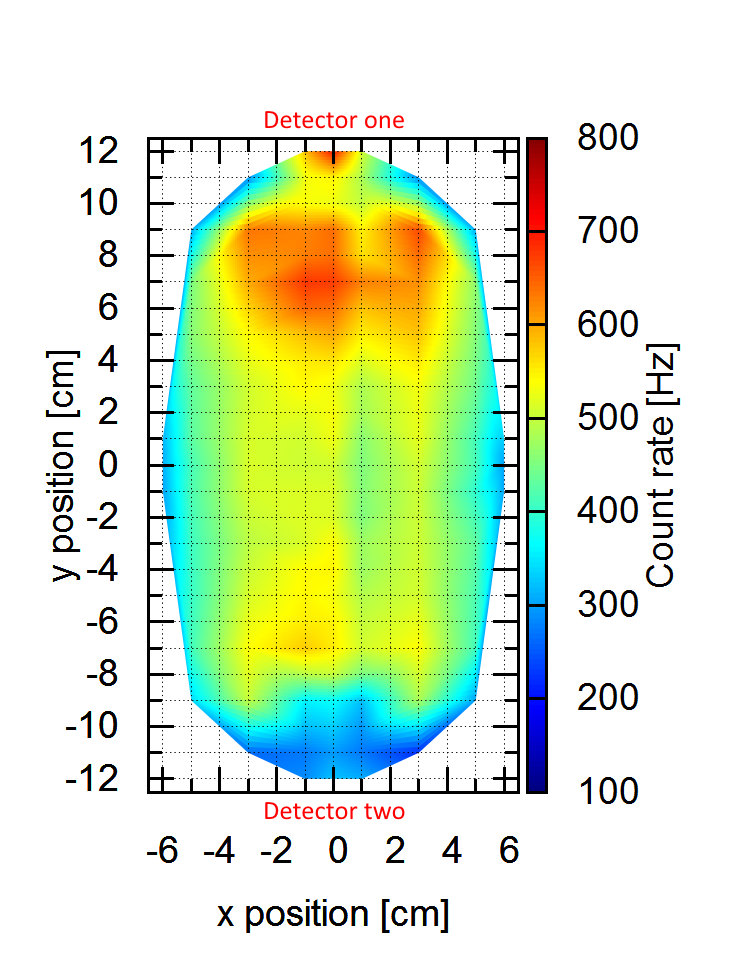
\includegraphics[width=0.4\textwidth]{./plots/spatial/Det1.png}}
	\hfill
	\subfloat[Detector two] {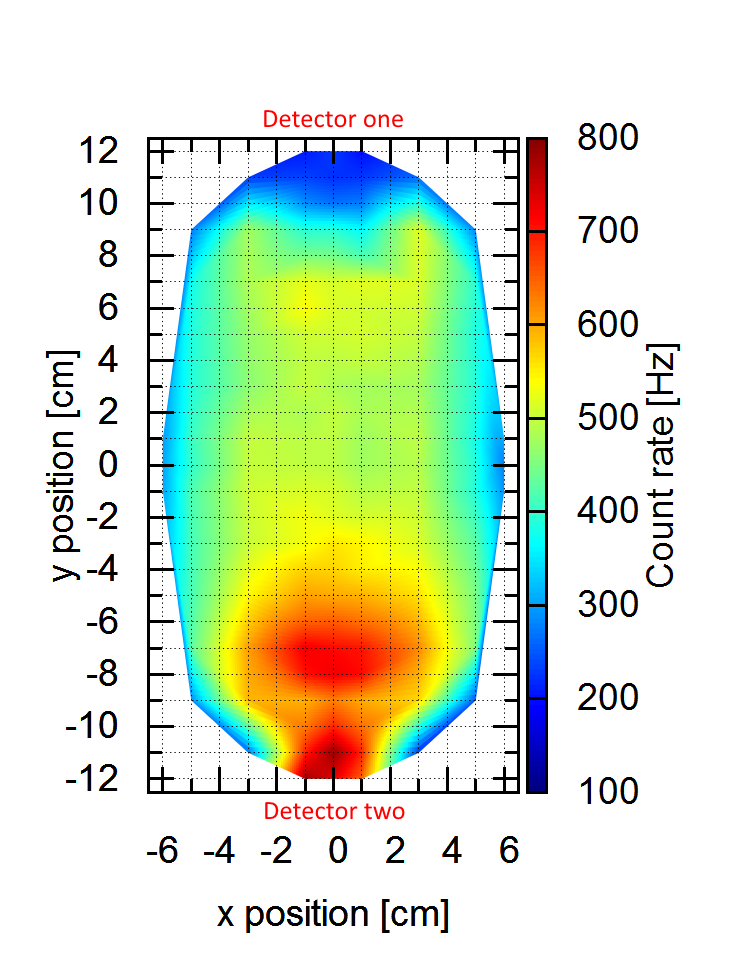
\includegraphics[width=0.4\textwidth]{./plots/spatial/Det2.png}}
	\hfill
	\subfloat[Coincidence rate] {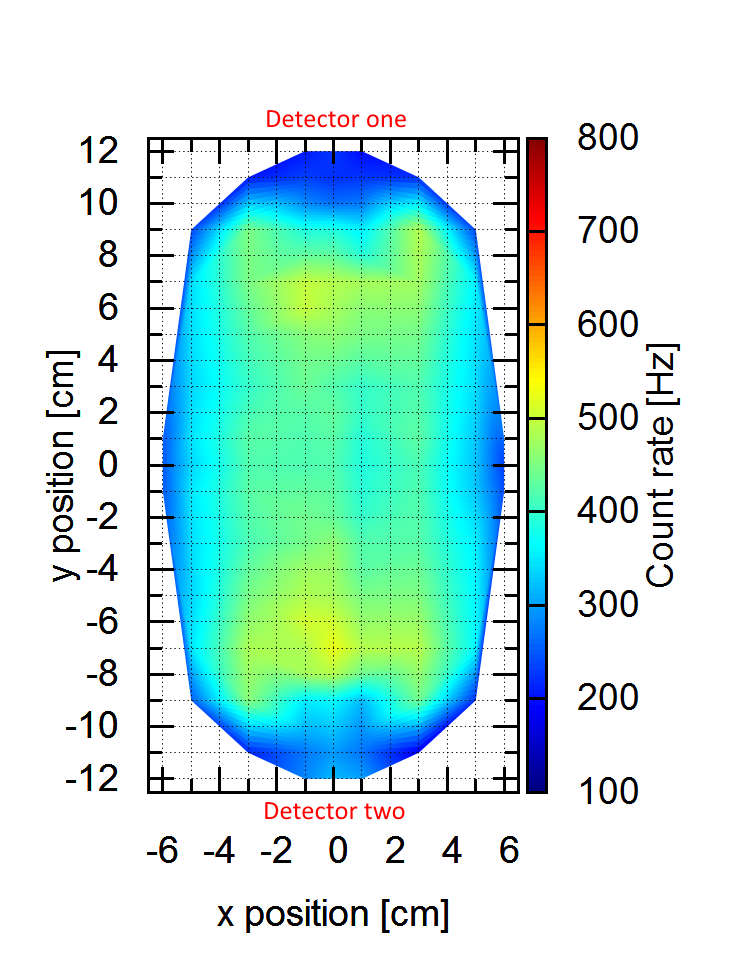
\includegraphics[width=0.4\textwidth]{./plots/spatial/Coinc.png}}
	\hfill
	\caption[Efficiency measurement setup]{Efficiency measurement at plastic scintillator with a \sr{} source at different positions. The heat map was plotted with \tit{gnuplot's pm3d} feature, the data between the measurement points was interpolated by the same software. Note that the coincidence count rate in front of one detector is mainly dominated by the count rate of the opposite detector.}
	\label{fig:ch5:efficiency}
\end{figure} 
\newpage
Nevertheless, the readout setup had to be changed to avoid walk (see figure \ref{fig:ch5:scheme_timing}). To do so, the leading edge discriminator was replaced by a \tit{constant fraction discriminator} (CF4000 from GSI, $\SI{1}{\nano\second}$ delay line, adjustable threshold and zero cancellation). Furthermore, a \tit{time to pulse height converter} (Ortec 437A) was installed to display the time differences between detector one and two as a pulse height. This necessitates signal one (start) to be definitely earlier than signal two (stop), so signal two was delayed with a constant delay (long cable, $\SI{50}{\nano\second}$). To avoid noise in the time spectrum, the coincident signal of one and two gated the TPC in order to just register events, in which the signals are coincident. The pulse height spectrum was digitized by a $13$-bit \tit{analog-to-digital converter} (Caen N957) and monitored by a \texttt{root}\footnote{\texttt{root}: data analysis framework by CERN \cite{root}} framework on a UNIX-system. \par
\begin{figure}[t!]
	\centering
	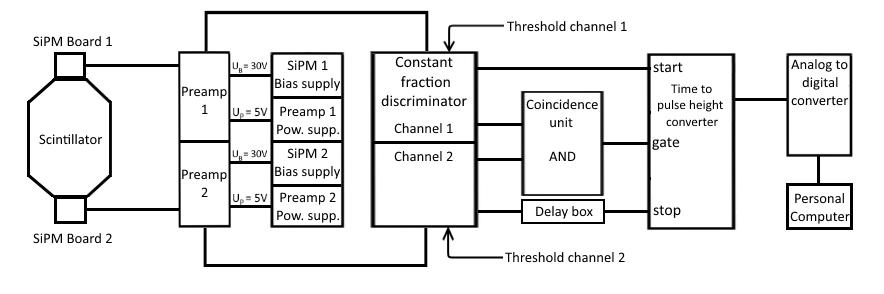
\includegraphics[width=1\linewidth]{./graphics/ch5/scheme_timing.png}
	\caption[Schematic of the time resolution measurement]{Setup of the time resolution measurement.}
	\label{fig:ch5:scheme_timing}
\end{figure} 
\begin{figure}[b!]
	\centering
	\subfloat[Time calibration spectrum. The second x-axis already shows the calibrated time. The key represents the employed delays.] {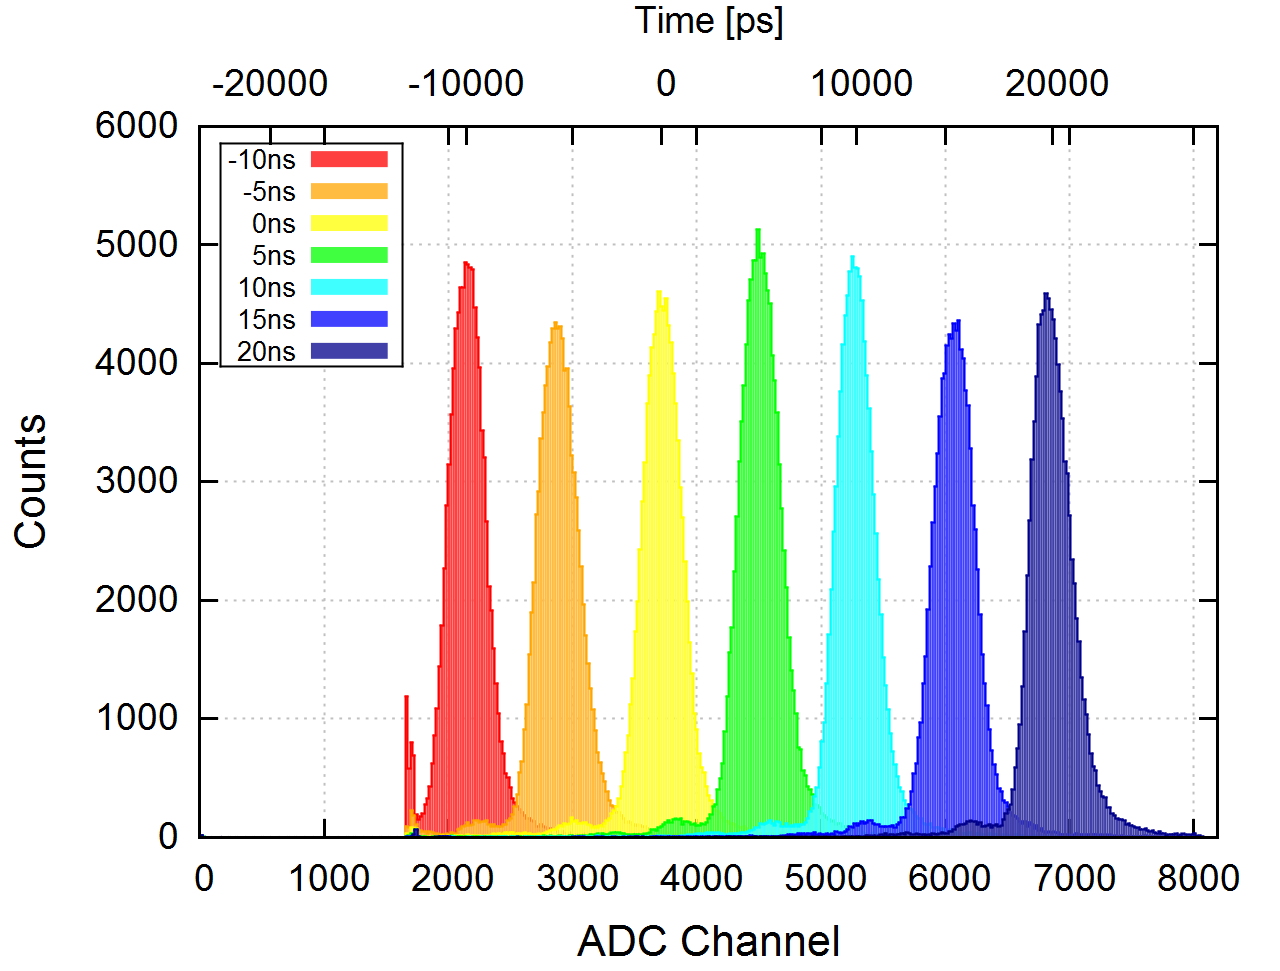
\includegraphics[width=0.49\textwidth]{./plots/timing/ze_hist.png}}
	\hfill
	\subfloat[Time calibration fit. The datapoints were extracted via Gaussian fits, using the \texttt{root} framework.] {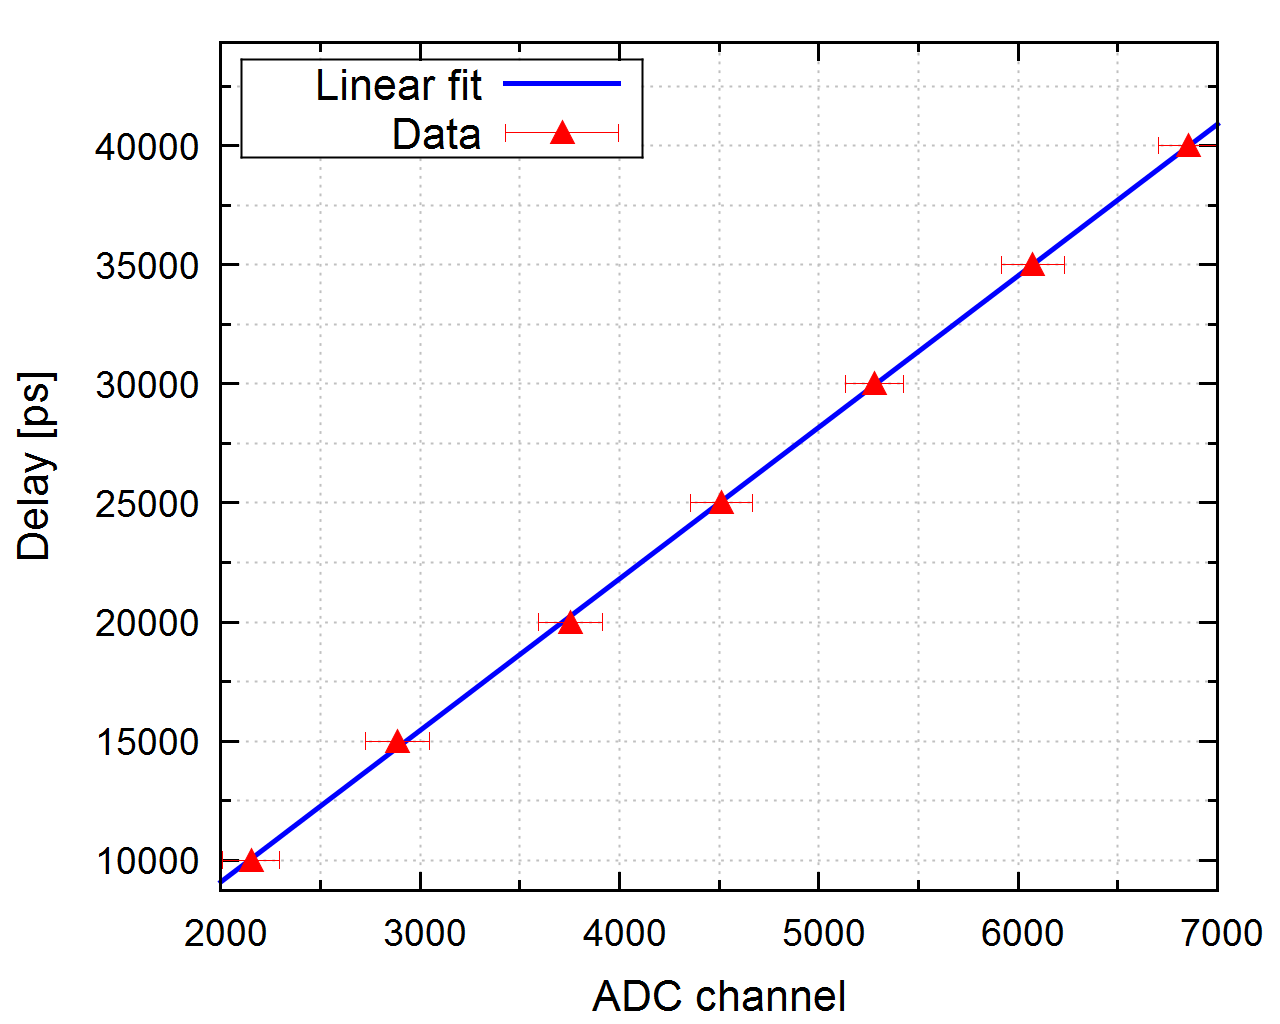
\includegraphics[width=0.49\textwidth]{./plots/timing/ze.png}}
	\hfill
	\caption[Time calibration]{Time calibration for different delays.}
	\label{fig:ch5:calibration}
\end{figure}
Since the net delay between signal one and two is random due to electronics and processing, a time calibration had to be made. For this, the \sr{} source was placed in the very middle of the scintillator (equally to the section before), so the time difference between coincident signals in detector one and two should be zero. By testing different delays with an adjustable delay box, the delay was set in a way that the peak of the resulting time spectrum was near the center of the acceptance of the ADC ($\approx$ channel 4000). By slightly increasing and decreasing the delay, the peak changes its position around the center. This yields a linear correlation between channel number $K$ and time $T$:
\begin{align*}
T(K)=\text{slope}\cdot K + T_0 = 6.3611\frac{\si{\nano\second}}{\text{ch}}\cdot K-23631\si{\nano\second}.
\end{align*}
The calibration spectrum and the linear fit are shown in figure \ref{fig:ch5:calibration}. The data for the linear fit was extracted by fitting Gaussians within the \texttt{root} framework to the peaks in the time spectrum. The error of each data point is given by the standard deviation of the Gaussian fit.\par      
Analog to the previous section, the \sr{} source was moved to different positions for determining the time resolution by measuring the standard deviation of the peak, and the propagation time by determining the position of the peak relative to the center. The threshold for both detectors was set to $\SI{-50}{\milli\volt}$, to detect the first incoming photons of each event for fastest response. 
This is visualized in figure \ref{fig:ch5:timing}. \par 
\begin{figure}[t!]
	\centering
	\subfloat[Measurement positions] {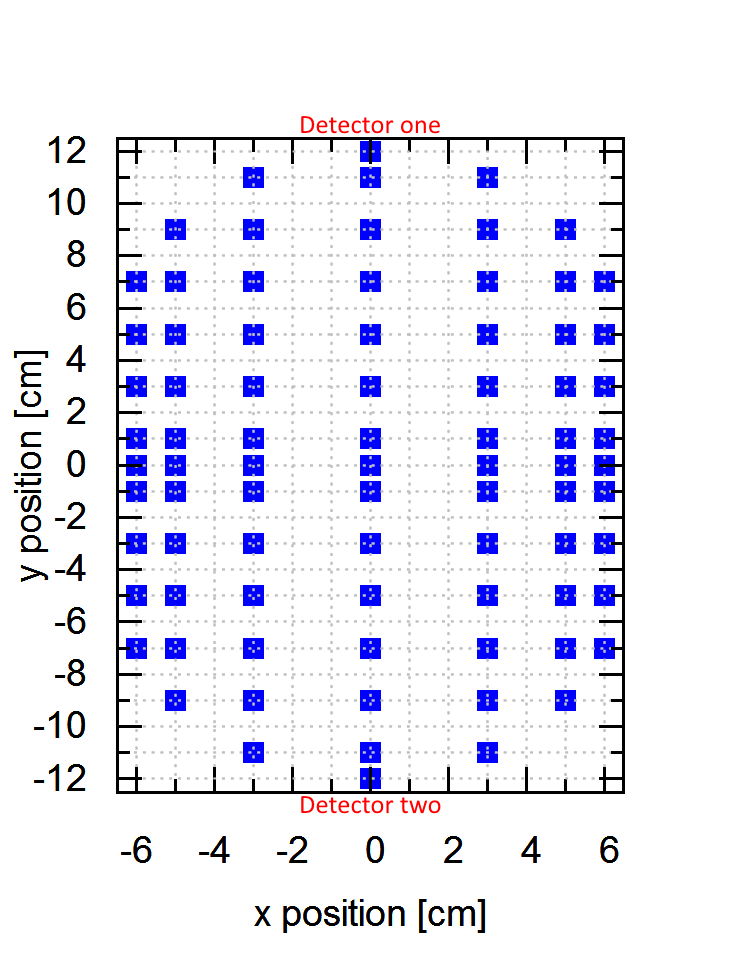
\includegraphics[width=0.33\textwidth]{./plots/timing/punkte.png}}
	\hfill
	\subfloat[Time resolution] {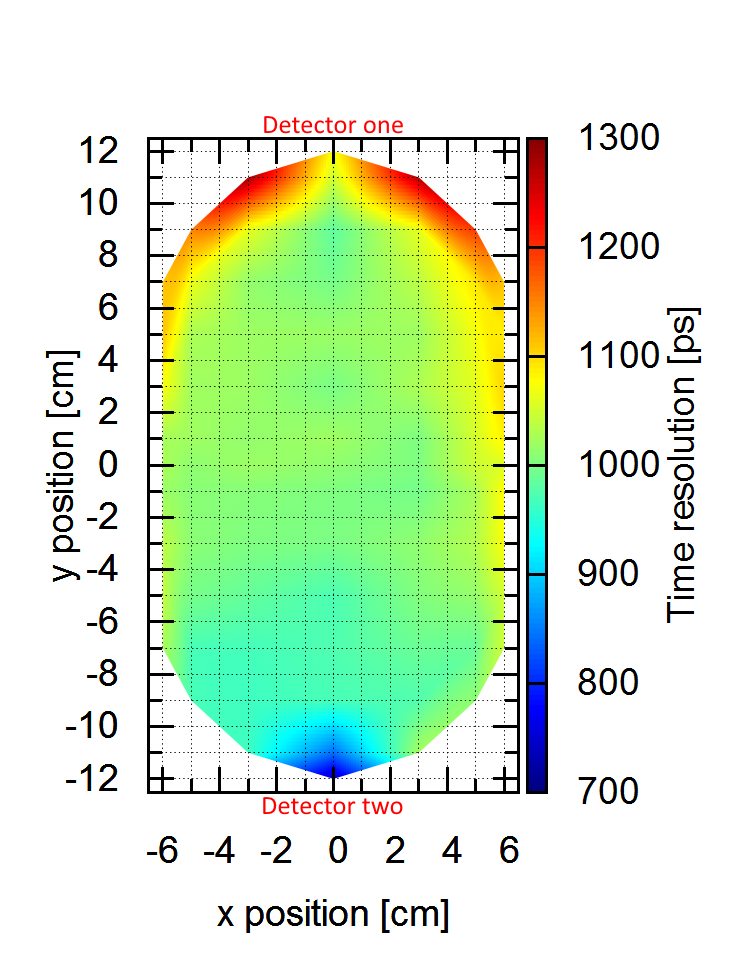
\includegraphics[width=0.33\textwidth]{./plots/timing/aufl.png}}
	\hfill
	\subfloat[Propagation time] {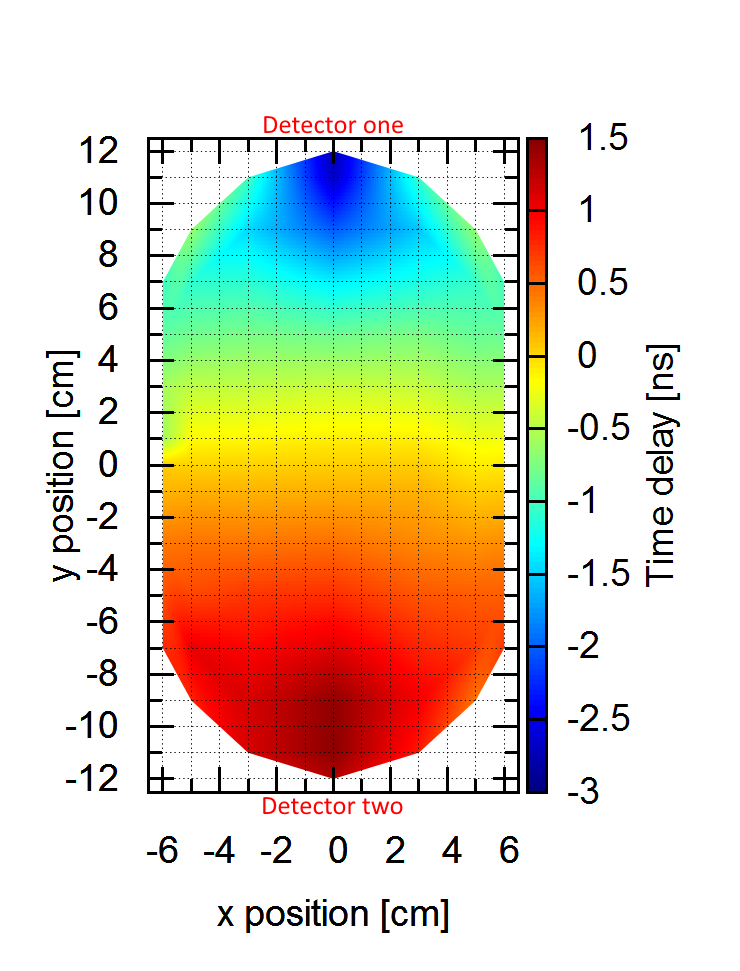
\includegraphics[width=0.33\textwidth]{./plots/timing/tof.png}}
	\hfill
	\caption[Timing reolution measurement]{Time resolution measurement at plastic scintillator with a \sr{} source at different positions. The heat map was plotted with \tit{gnuplot's pm3d} feature, the data between the data points was interpolated by the same software.}
	\label{fig:ch5:timing}
\end{figure}
Again, an obvious asymmetry can be observed. The time resolution right in front of detector two is best with approximately $\SI{700}{\pico\second}$ and rises to $\SI{1}{\nano\second}$ in the center of the scintillator. The resolution stays nearly stable but deteriorates towards the edges near detector one. \par 
This behavior is more pronounced when investigating the propagation time of the scintillation light. The theoretical propagation time for photons in medium is given by 
\begin{align}
T=\frac{s}{n^{-1}\cdot c_0},
\end{align}
where $s$ is the length, $n$ the refractive index ($n=1.58$ EJ-248M \cite{eljen}) for the medium and $c_0$ the speed of light in vacuum. Therefore, one expects
\begin{align*}
T_{\text{max}}=\frac{\SI{0.25}{\meter}}{1.58^{-1}\cdot\SI{299792458}{\meter\per\second}}\approx\SI{1300}{\pico\second}
\end{align*}
as the maximum propagation time, when the source is placed right in front of one detector. This can be found for detector two. Still, detector one shows nearly three times the expected result. \par 
\begin{figure}[t!]
	\centering
	\subfloat[The left peak represents the y position over detector one, right peak over detector two. The time distance between two peaks should represent the maximum propagation time of the photons.] {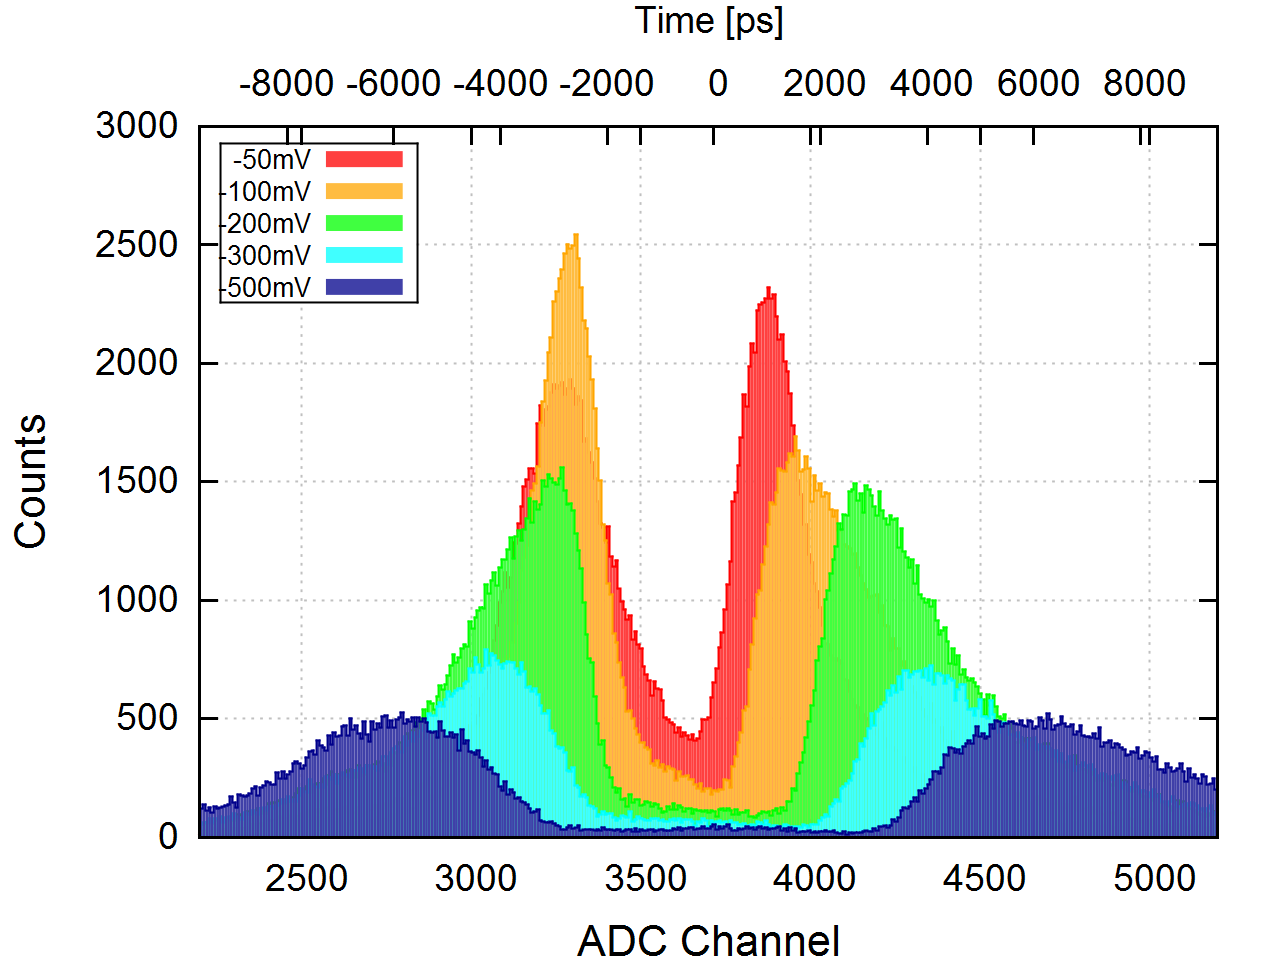
\includegraphics[width=0.49\textwidth]{./plots/timing/abst_hist.png}}
	\hfill
	\subfloat[Difference of relative timing between the detectors for the two extreme positions of the source] {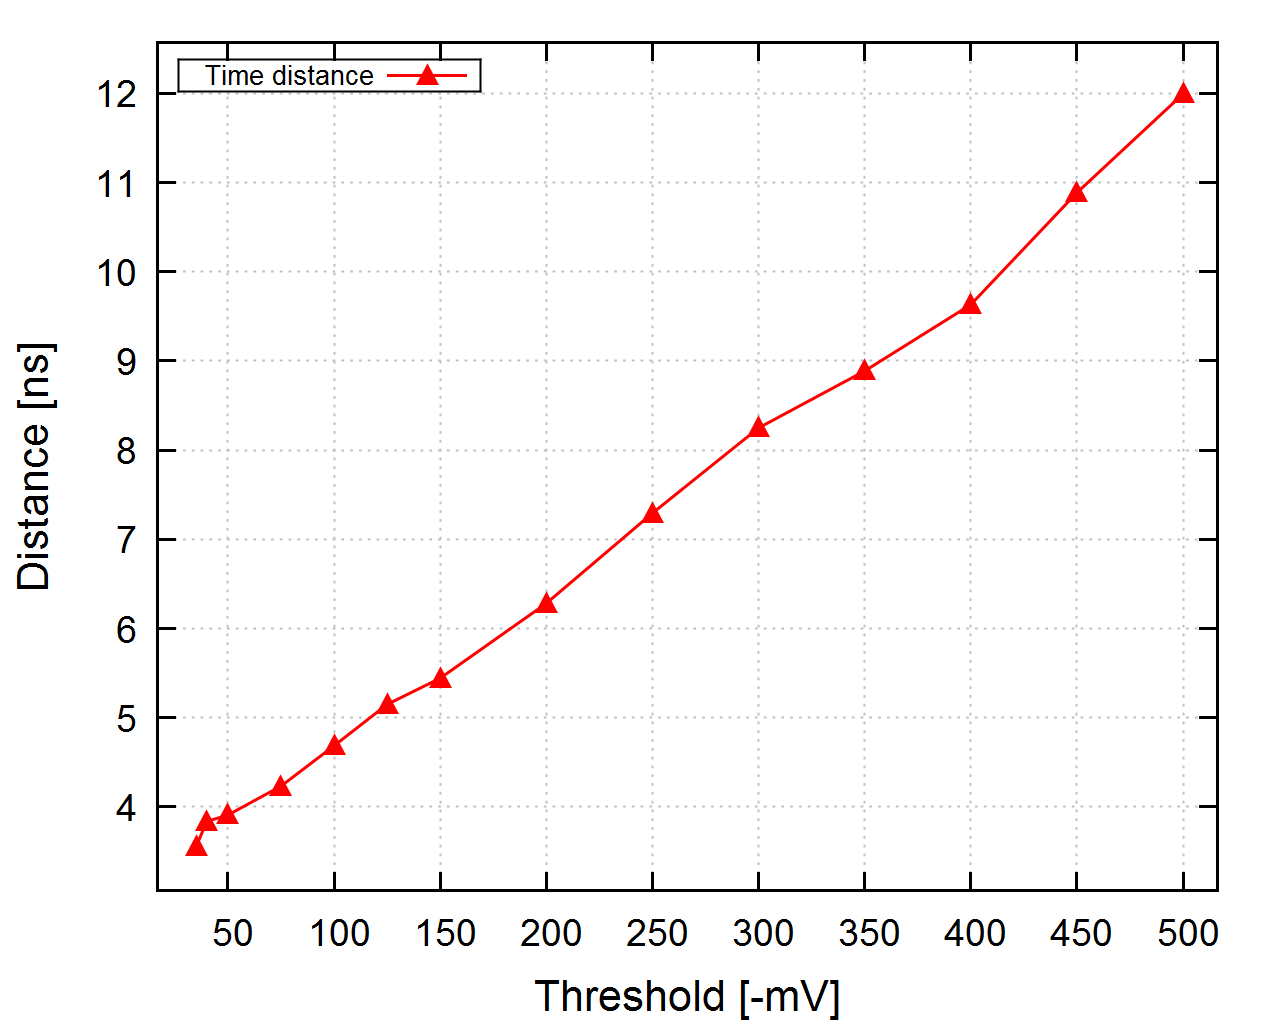
\includegraphics[width=0.49\textwidth]{./plots/timing/abst.png}}
	\hfill
	\caption[Threshold dependence of the propagation time measurement]{Threshold dependence of the propagation time measurement.}
	\label{fig:ch5:threshold_dependenecy}
\end{figure}
To study this asymmetry, the threshold of both detectors was increased. A higher threshold suppresses the first photons arriving at the detector since they produce only a small signal. To overcome this, more photons are needed, so a signal is only generated when reflected photons are adding up to the signal as well, leading to a longer propagation time. Hence, for higher thresholds more delay can be expected. To show this behavior, the source was placed above detector one and then above detector two. The resulting time should be the travel time of photons for $2\times\SI{25}{\centi\meter}$ in the scintillator material and is represented by the horizontal distance of the two peaks plotted in figure \ref*{fig:ch5:threshold_dependenecy}. For $\SI{-50}{\milli\volt}$, the right peak (represents detector two) is ca. $\SI{1.5}{\nano\second}$ off center and satisfies the calculations. This can also be seen in figure \ref{fig:ch5:timing}b. The left peak, representing detector one, shows nearly $\SI{2.5}{\nano\second}$ delay. The peak of detector two moves to higher delays, which is expected due to reflections, whereas the peak for detector one stays at the same position until a threshold of $\SI{-300}{\milli\volt}$. For this and higher thresholds the peaks are distributed symmetrically to the y-axis. Still, this symmetry should occur for all thresholds. \par
An explanation for the asymmetry in the efficiency, time resolution and propagation time measurements might be dissimilar sensitivities of the two detectors. A good resolution is achieved when both detectors are exposed to a high amount of direct light, so seeing less direct light results in bad timing. One can assume, and the efficiency measurements confirms this, that, when the source is placed right in front of one detector, this detector sees sufficient direct light. Hence, bad timing in front of one detector is due to bad performance of the opposite detector. Therefore, detector one seems to perform better than its counterpart. \par 
\begin{figure}[t!]
	\centering
	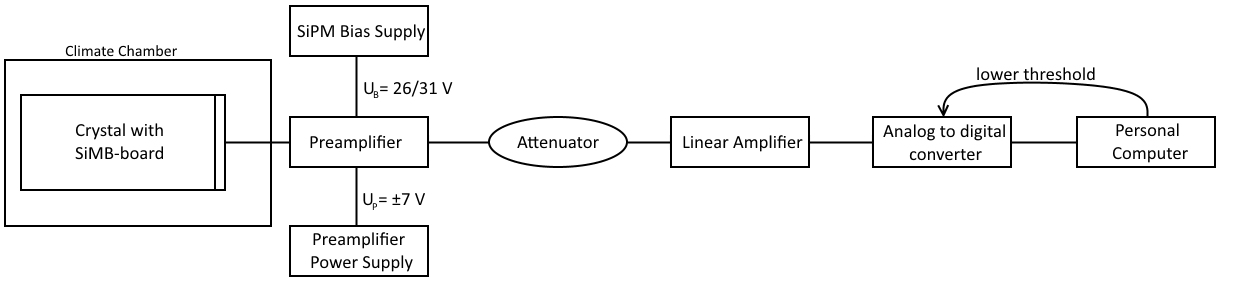
\includegraphics[width=1\linewidth]{./graphics/ch5/scheme_energy.png}
	\caption[Schematic of the energy measurements]{Schematic of the energy measurements}
	\label{fig:ch5:scheme_energy}
\end{figure}
This problem might be overcome by fine tuning the thresholds and gains (biasing) of the detectors. To refer to figure \ref{fig:ch5:threshold_dependenecy}, the left peak represents the allegedly good working detector one. By rising the threshold, the peak remains at the same position until a certain level is exceeded. This might be an indicator that at this very point the reflected light dominates. This cannot be seen for detector two: a saturation where the peak is stable for distinct thresholds was not found. \par 
Further work on tuning the setup parameters as well as using up to date processing electronics might lead to a distinct increase in precision. 

\section{Energy measurements}

\begin{figure}[t!]
	\centering
	\subfloat[LYSO crystal, sized $\SI{10}{\milli\meter}\times\SI{10}{\milli\meter}\times\SI{3.5}{\milli\meter}$] {\includegraphics[width=0.49\textwidth]{./pictures/Crystal/lyso.jpg}}
	\hfill
	\subfloat[\pwo{} crystal (sized $\SI{20}{\milli\meter}\times\SI{20}{\milli\meter}\times\SI{50}{\milli\meter}$) with the $3\times 2$ matrix-board] {\includegraphics[width=0.49\textwidth]{./pictures/Crystal/lyso_board.jpg}}
	\hfill
	\caption[LYSO and \pwo{} crystals]{LYSO and \pwo{} crystals with the $3\times 2$ matrix SiPM-board.}
	\label{fig:ch5:crystals}
\end{figure}

Another application for SiPMs could be the usage in calorimetry, measuring deposited energy of particles in scintillators. Some prominent inorganic scintillator crystals were used, LYSO ($\SI{10}{\milli\meter}\times\SI{10}{\milli\meter}\times\SI{3.5}{\milli\meter}$) and \pwo{} ($\SI{20}{\milli\meter}\times\SI{20}{\milli\meter}\times\SI{50}{\milli\meter}$), to measure several $\gamma$-spectra from calibration sources. \par 
The small LYSO crystal was equipped with a $2\times 1$ parallel SiPM-configuration. The board was attached with optical grease to the $\SI{10}{\milli\meter}\times\SI{10}{\milli\meter}$ surface, the other sides of the crystal were covered with reflective tape. For stability and lightproofing, this combination was then wrapped in black tape. \par 
The \pwo{} crystal was wrapped in eight layers of Teflon foil, one thin layer of aluminum foil and fixed with shrinking tube, leaving the front surface ($\SI{20}{\milli\meter}\times\SI{20}{\milli\meter}$) uncovered. On this side, a $3\times 2$ parallel SiPM-configuration was attached analogous to previous setups, see figure \ref{fig:ch5:crystals}. \par
Using a \textit{KETEK} preamplifier \cite{ketek_preamp}, the crystals were set up in the climate chamber (\tit{WEISS}, see figure \ref{fig:ch5:scheme_energy}). The amplified signal was further shaped by a linear amplifier (Ortec 410) with adjustable integration time and gain. The energy spectrum was taken by an analog-to-digital converter from Caen (N957) which was controlled by a UNIX-workstation. \par   

\subsection{LYSO}
First, the LYSO crystal was tested at $\SI{-25}{\degreeCelsius}$ under $\gamma$-radiation from a \co{} source. It appeared that the raw signal of the two SiPMs in parallel was so strong that the preamplifier saturated, so the bias voltage was set to $\SI{26}{\volt}$ right beyond breakdown. The same problem with the linear amplifier was solved by using a $\SI{-20}{\decibel}$ passive attenuator. By choosing $\SI{2}{\micro\second}$ integration time and a proper amplification, the gain was set in a way that the photopeaks of \co{} were between channel 5000 and 6000 to use the full range of the $13$-bit analog-to-digital converter.  \par  
Consecutively, the energy spectra of several calibration sources (\co{}, \na{}, \cs{}, \ba{} and \eu{}) were taken. To calibrate the setup, the most prominent photopeaks were fitted with Gaussians. The calibration fit is depicted in figure \ref{fig:ch5:lyso_eichung}, the spectra are plotted in figure \ref{fig:ch5:lyso_energy}. The same procedure was done at $\SI{25}{\degreeCelsius}$, where the amplification of the linear amplifier had to be increased by a factor of 4. \par 
The photopeak of \ba{} is distinct as well as the x-ray peak at low energies. The cobalt spectrum has a large compton background since the gamma quanta with $\SI{1.1}{\MeV}$ and $\SI{1.3}{\MeV}$ (all gamma ray energy data is retrieved from \cite{gamma_energy}) are too energetic to be fully stopped in the $\SI{3.5}{\milli\meter}$ thick crystal. For this, the two photopeaks are barely visible, the sum peak could not be observed at all. Furthermore, \cs{} and \na{} show a clear photopeak and a distinct compton spectrum, the $\SI{511}{\keV}$ peak due to annihilation of the positron from the $\beta^+$ decay of sodium is clearly visible. The \eu{} source was tested as a calibration source since the spectrum shows multiple gamma energies and it was found that the most prominent peaks ($\SI{344}{\keV}$, $\SI{244}{\keV}$, $\SI{121}{\keV}$, $\SI{40}{\keV}$) could be resolved, especially for $\SI{-25}{\degreeCelsius}$. More detailed energy spectra plots can be found in \ref{ap:energy_spectra}.  \par 
The energy resolution $R$, defined as the ratio of \tit{full width at half maximum} (FWHM) and photoenergy, was calculated as well. The whole data is given in \ref{ap:B:tab:energy_spectra}. The resolution is plotted in figure \ref{fig:ch5:lyso_resolution}. The resolution of the cooled system is in some cases ($\SI{300}{\keV}$ to $\SI{700}{\keV}$) slightly better. For low and high energies, larger errors can be found. 
\par 
\begin{figure}[t!]
	\floatbox[{\capbeside\thisfloatsetup{capbesideposition={left,center},capbesidewidth=0.45\linewidth}}]{figure}[\FBwidth]
	{\caption[Energy resolution for the LYSO crystal setup]{Energy resolution for the LYSO crystal setup. The photo peaks for $\SI{244.7}{\keV}$ and $\SI{1173.2}{\keV}$ were not distinct at $\SI{25}{\degreeCelsius}$ and therefore were not fitted. Hence, some of the error bars are large. }    
		\label{fig:ch5:lyso_resolution}}
	{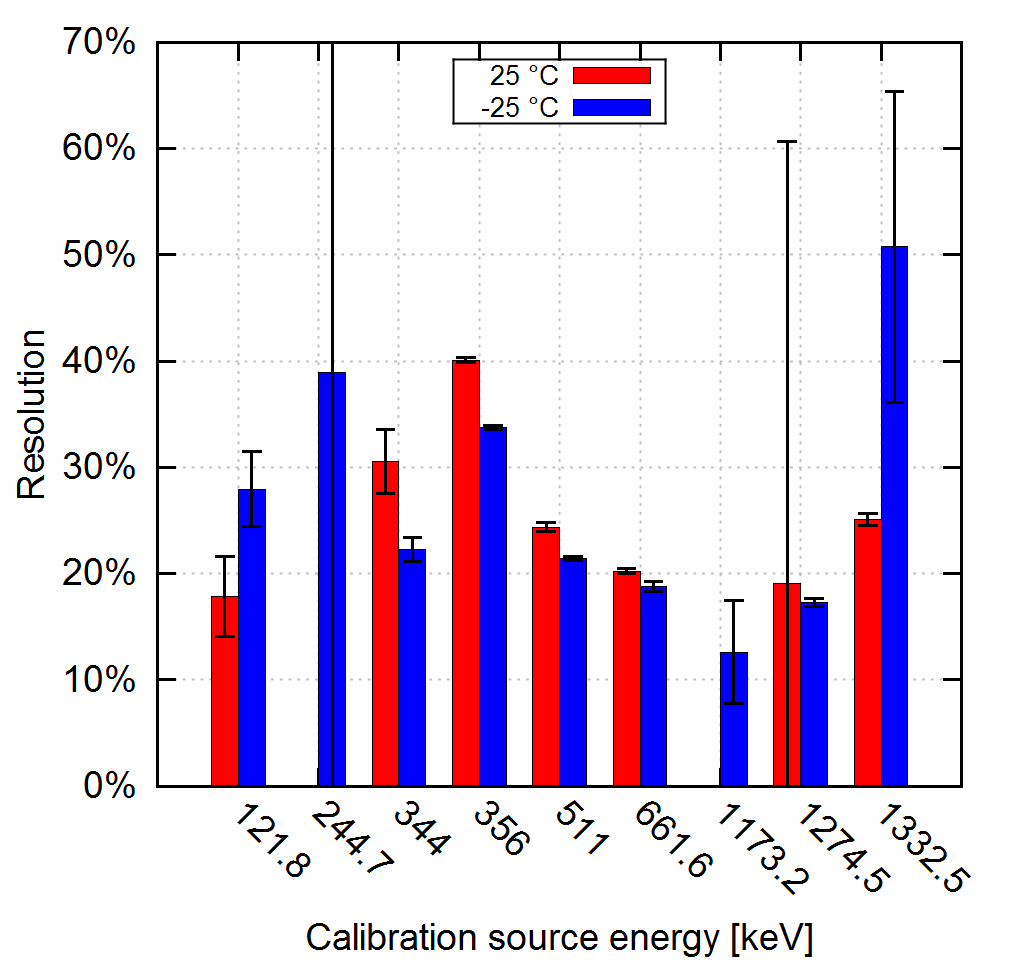
\includegraphics[width=0.55\textwidth]{./plots/energy/lyso_resolution.png}}
\end{figure} 
Cooling does not seem to improve the energy reolution significantly, despite the intrinsic dark noise of the SiPM is suppressed and the light yield of the scintillator is improved. The strong raw signal indicates that a lot of scintillation light is seen by the SiPMs. 
\begin{figure}[H]
	\centering
	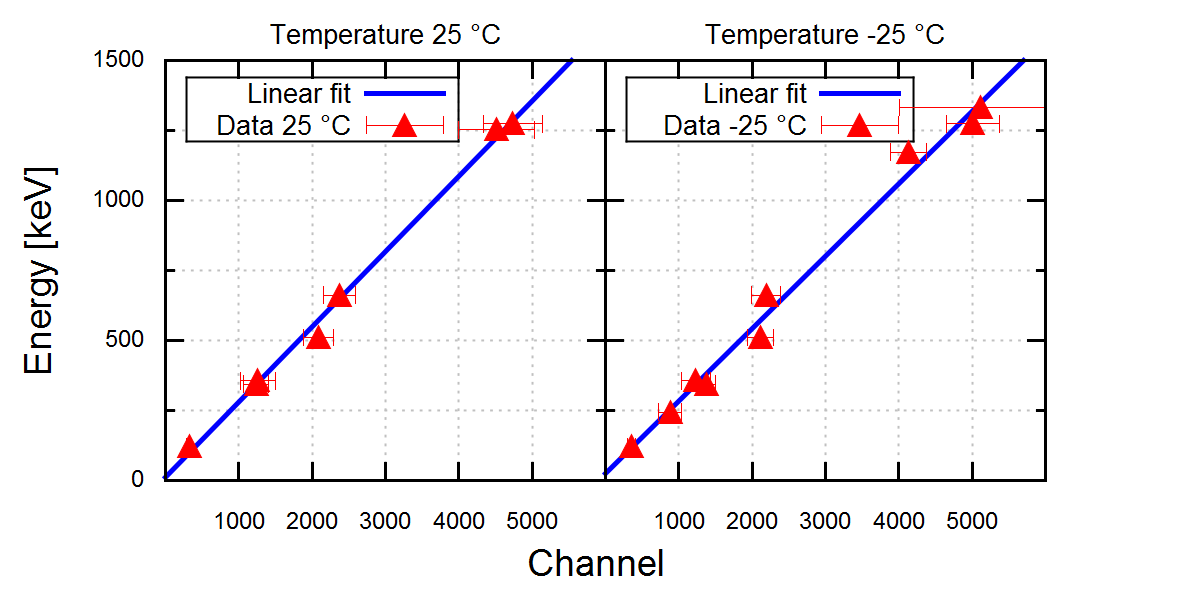
\includegraphics[width=1\linewidth]{./plots/energy/lyso_eichung.png}
	\caption[LYSO energy calibration]{Energy calibration with different sources using the LYSO crystal.}
	\label{fig:ch5:lyso_eichung}
\end{figure} 
\begin{figure}[H]
	\centering
	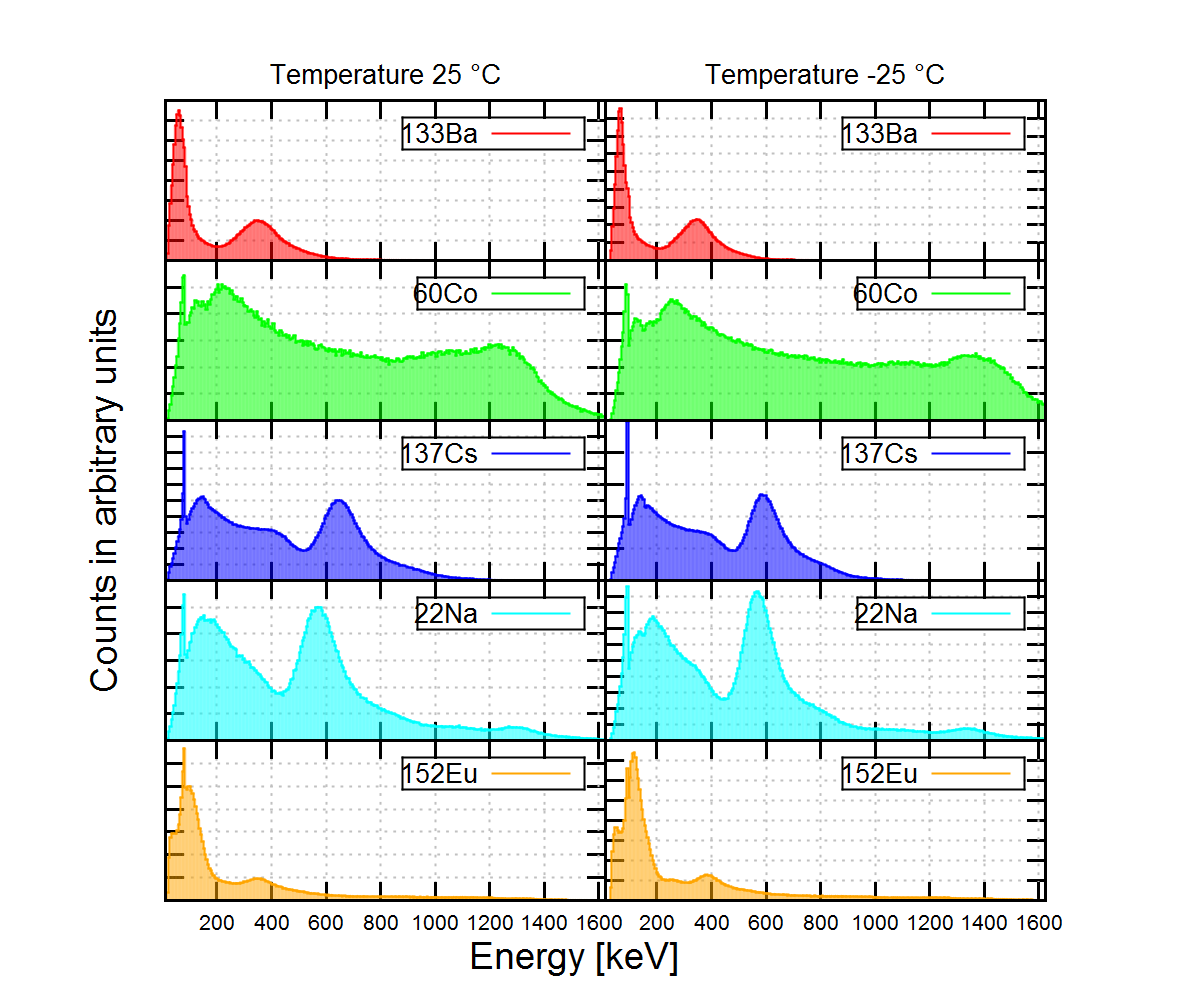
\includegraphics[width=1\linewidth]{./plots/energy/lyso_energy.png}
	\caption[LYSO energy spectra]{Energy spectra of several calibration sources using the LYSO crystal.}
	\label{fig:ch5:lyso_energy}
\end{figure}
\newpage
\noindent
According to table \ref{ch2:tab:characteristics}, LYSO is a very bright scintillator with 30000 photons per $\SI{511}{\keV}$ photon, even higher when cooled. The SiPMs seem to be overexerted due to this large amount of photons. This might be solved by a higher number of microcells (smaller pixel size), so more photons can be detected at the same time. This overextension could be the reason why cooling does not result in a significant better resolution. Still, an improvement by cooling is expected for crystals with lower light yield, i.e. lead tungstate, which will be covered in next section.      

\subsection{\pwo{}}

The lead tungstate setup with six parallel SiPMs is operated comparable to the LYSO setup with two SiPMs. However, the light yield of \pwo{} is several orders of magnitude lower (\ref{ch2:tab:characteristics}) than LYSO, and roughly $85-110$ photons per $\si{\MeV}$ are expected \cite{panda_emctdr}.\par 
\begin{figure}[b!]
	\centering
	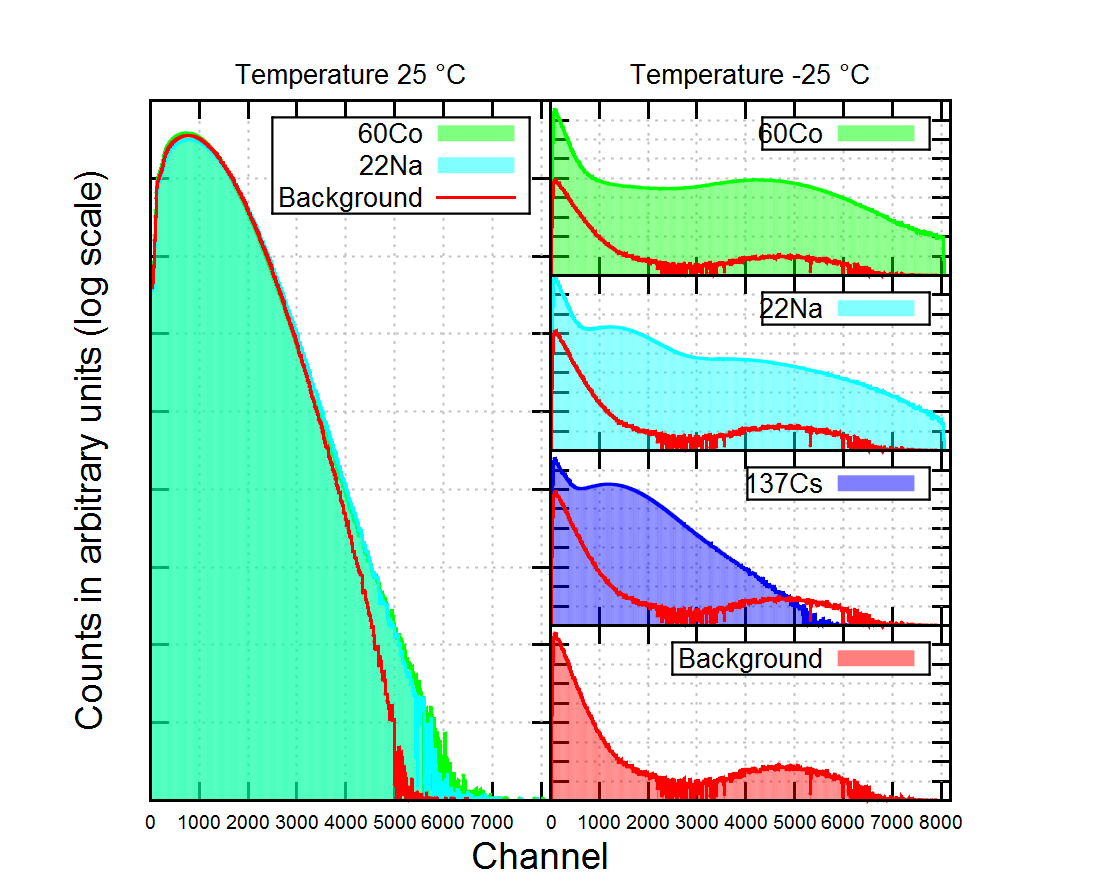
\includegraphics[width=1\linewidth]{./plots/energy/pwo_energy.png}
	\caption[\pwo{} energy spectra]{\pwo{} energy spectra of several calibration sources.}
	\label{fig:ch5:pwo_energy}
\end{figure}
Figure \ref{fig:ch5:pwo_energy} shows the energy spectra of several calibration sources. At higher temperature ($\SI{25}{\degreeCelsius}$), the energy spectra merge with the background. At this point, one has to consider the \tit{photo detection efficiency} (PDE) of the SiPMs ($\approx 40\%$) for the emission wavelength of \pwo{} ($\SI{425}{\nano\meter}$), the loss of photons due to absorption ($\approx 10\%$) and the effective light sensitive area (ratio of the sensitive area of the SiPM and the $\SI{20}{\milli\meter}\times\SI{20}{\milli\meter}$ crystal surface, about $13.5$\%). Hence, only few photons are left, diminishing the resolution of the spectrum. The measurements at $\SI{25}{\degreeCelsius}$ show that only for a small amount of events a sufficient number of photons are registered to fill bins beyond the background. However, this is not sufficient for determining the particle energy. \par 
The spectra at $\SI{-25}{\degreeCelsius}$ are more distinct: \co{} shows a broad and flat peak in which the two photopeaks are merged. The \na{} spectrum shows both the annihilation peak and the photopeak at $\SI{1275}{\keV}$, so does the \cs{} spectrum at $\SI{662}{\keV}$. The background shows less noise compared to the background at $\SI{25}{\degreeCelsius}$. Reason being the higher light yield ($\approx \times 3.5$ \cite{panda_emctdr}) and the suppressed thermal noise of the SiPMs. A small peak at channel 5000 is also visible and will be discussed in the following section. \par 
\subsection{Muons}
The \pwo{} setup was also used to measure the energy deposit of cosmic muons in lead tungstate. According to \cite{panda_emctdr}, the energy deposit for minimum ionizing particles is $\SI{10.2}{\MeV\per\centi\meter}$, so one expects a mean energy loss of $\approx \SI{20}{\MeV}$ in the crystal with a thickness of $\SI{2}{\centi\meter}$. Since the energy deposit of cosmic muons in matter varies due to the statistical nature of the energy loss, whose mean value is given by the Bethe-Bloch-formula (see equation \eqref{eq:bethe_bloch}), a Landau distribution with a peak at $\approx \SI{20}{\MeV}$ is expected. \par 
Since the light yield is higher and the noise is suppressed at low temperatures, the \pwo{} was cooled down to $\SI{-25}{\degreeCelsius}$. A \co{} spectrum was taken to calibrate the range of the analog-to-digital converter, the spectrum can be seen in figure \ref{fig:ch5:muon_spectrum}. The gain was adjusted to set the energy range of the ADC from $\SI{0}{\MeV}$ to $\SI{40}{MeV}$. After removing the calibration source, data was taken for $\SI{48}{\hour}$ due to the small flux of muons through the crystal. The resulting spectrum is shown in the same figure.  \par 
A large background can be found in the first 2000 channels. By comparison with the calibration spectrum of \co{}, it appears that several other gamma sources, either intrinsic or natural environmental radiation, with energies up to $\SI{2}{\MeV}$ contribute to the muon spectrum. A possible candidate is \ka{} with a gamma energy of $\SI{1460.9}{\keV}$, which not only is present in the environment but also as part of the crystal (impurity, up to $0.48$ ppm \cite{analytical_report}). The muon spectrum itself is broad and flat and shows no Landau distribution at all. This might be caused by the geometry of the setup when muons travel through more or less than $\SI{2}{\centi\meter}$ of crystal and hence lose not exactly $\SI{20}{\MeV}$ of energy. This could cause the spectrum to show no distinct Landau peak. \par 
\begin{figure}[b!]
	\centering
	\subfloat[Energy spectrum without any trigger and small range] {\includegraphics[width=0.49\textwidth]{./plots/energy/Muons_ohne_Trigger.png}}
	\hfill
	\subfloat[Energy spectrum with upper and lower trigger and wide range] {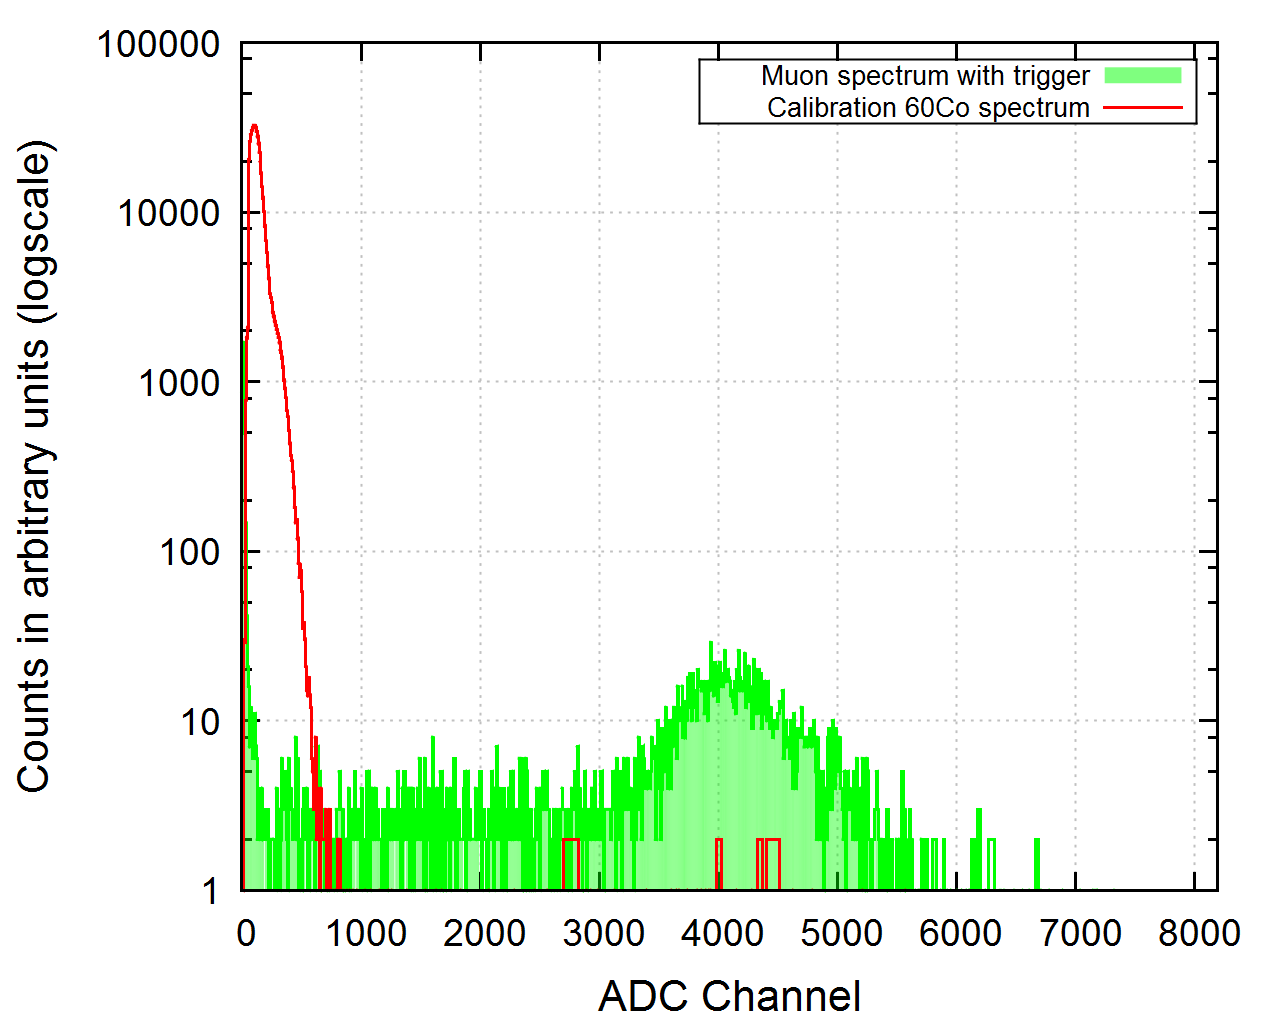
\includegraphics[width=0.49\textwidth]{./plots/energy/muon_both_trigger.png}}
	\hfill
	\caption[Energy loss spectrum of cosmic muons]{Energy loss spectrum of cosmic muons. Picture (a) shows a large intrinsic background.}
	\label{fig:ch5:muon_spectrum}
\end{figure}
As a solution for this problem, a trigger system  consisting of two plastic scintillator bars with photomultiplier tube readout was utilized. Using one bar as an upper and one bar as a lower trigger, the two plastics were placed above and under the \pwo{} crystal. The coincident trigger signal gates the ADC, therefore only events measured in all three scintillators were added to the spectrum. The data is plotted in figure \ref{fig:ch5:muon_spectrum}. \par 
The first set of data, plot (a), was taken with a smaller energy range and without trigger system. The calibration spectrum was set to roughly $\SI{1200}{\keV}$ at channel 400, using the double peak of \co{}. The trigger system was then introduced since no peak could be observed and due to the large background. Plot (b) shows that the energy range is larger than before whereas the calibration peak could not be used as intended because of the nonlinearity of the ADC in small channel values. A peak at channel 4000 can be observed and the Landau distribution can be guessed. At lower channels (200 to 3000), smaller energy values due to geometrical effects are visible, for the plastic scintillator bars are larger as the \pwo{} crystal and therefore transition paths smaller than $\SI{2}{\centi\meter}$ are possible for muons.  






  



